\documentclass[oneside,a4paper, 12pt]{article}
\usepackage{anysize}
%\marginsize{left}{right}{top}{bottom}
\marginsize{2cm}{2cm}{1cm}{2cm}
\usepackage{long-geodesic}

\hypersetup{pdftitle={Long geodesics on convex surfaces},
pdfauthor={Arseniy Akopyan and Anton Petrunin}}

%\usepackage{lineno}\linenumbers

\begin{document}

\title{Long geodesics on convex surfaces}
\author{Arseniy Akopyan\thanks{Institute of Science and Technology Austria (IST Austria), Am Campus 1, 3400 Klosterneuburg, Austria} \and Anton Petrunin}
\date{}
\maketitle

\begin{abstract}
We review the theory of intrinsic geometry of convex surfaces in the Euclidean space and prove the following theorem: 
if the surface of a convex body $K$ contains arbitrary long closed simple geo\-de\-sics, then $K$ is an isosceles tetrahedron.
\end{abstract}

% \begin{figure}
% {r}{21 mm}
% \begin{lpic}[t(-4 mm),b(-0 mm),r(0 mm),l(0 mm)]{pics/long-geodesic(1)}
% \end{lpic}
% \end{figure}

\section{Introduction}
The goal of this note is to introduce the reader to the theory of intrinsic geometry of convex surfaces.
We illustrate the power of the tools by proving a theorem.

\begin{thm}{Theorem}
	\label{Long geodesic}
Assume that the surface $\Sigma$ of a convex body $K$ in the Euclidean space $\EE^3$
admits an arbitrary long simple closed geodesic.
Then $K$ is an isosceles tetrahedron.
\end{thm}

Let us remind that a curve in a surface is called \emph{geodesic} if every sufficiently short arc of the curve is length minimizing; if in addition it has no self intersections, we call it \emph{simple geodesic}.
A tetrahedron with equal opposite edges will be called \emph{isosceles}.

This theorem is extension of result of Vladimir Protasov~\cite{protasov2008onthenumber}, who proved it in assumption that $\Sigma$ is the surfaces of a convex polyhedron.
The advantage of the method of Alexandrov geometry is that it allows us to work with metrics of convex surfaces even they are not polyhedra, smooth manifolds or not equipped with any other convenient structure.

\begin{center}
	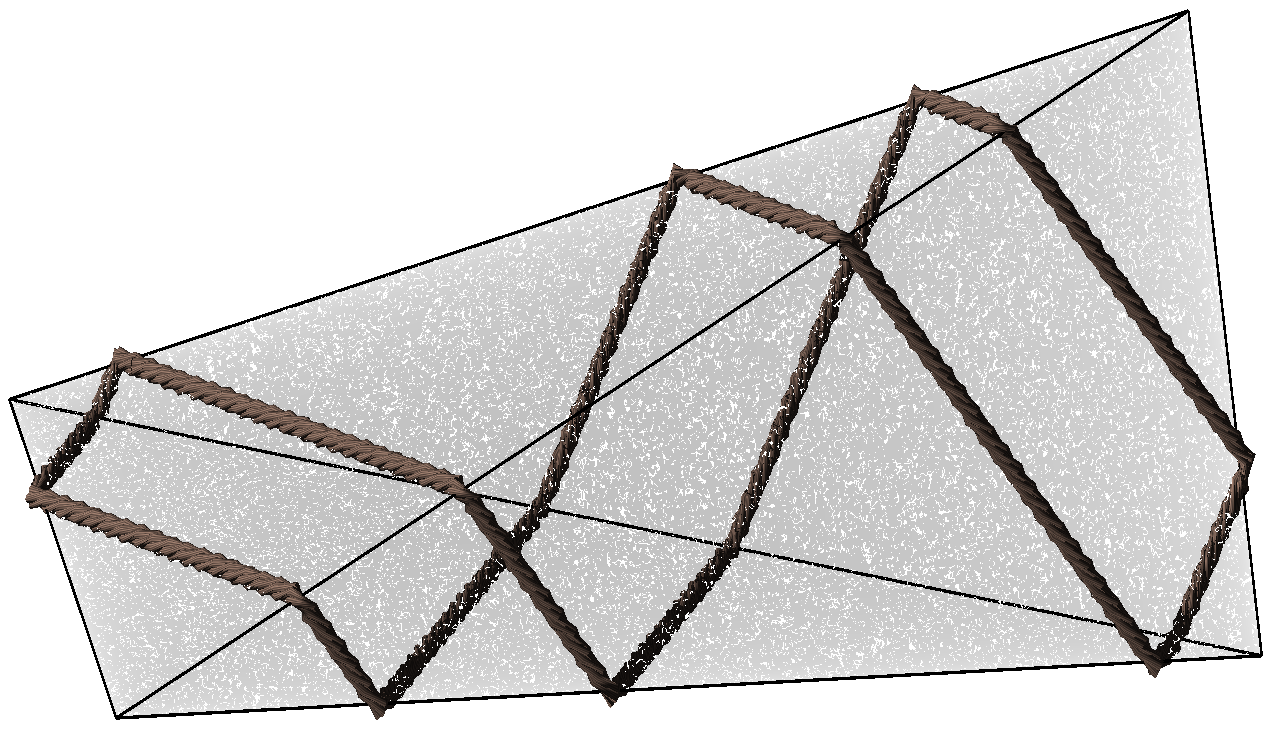
\includegraphics{pics/snow.png}\\
	Isosceles tetrahedron with closed geodesic on it.
	\label{fig:isoceles tetrahedron}
\end{center}


\section{An overview of the theory}

\begin{wrapfigure}[4]{r}{21 mm}
\begin{lpic}[t(-6 mm),b(0 mm),r(0 mm),l(0 mm)]{pics/cosine-rule(1)}
\lbl[t]{10,1;$a$}
\lbl[br]{5.5,9.5;$b$}
\lbl[bl]{16,9;$c$}
\lbl[bl]{7,4;$\gamma$}
\end{lpic}
\end{wrapfigure}

The geometry of intrinsic metric on convex surfaces
can be considered as generalization of Euclidean plane geometry,
where instead of equality in the cosine rule we have the following inequality
\[c^2\le a^2+b^2-2\cdot a \cdot b\cdot \cos\gamma.\]
This approach provides a uniform way to work with smooth and singular surfaces.

As the main reference, we will use the classical  book of Alexandrov \cite{aleksandrov1948vnutrennnyaya}; it is available in Russian and German.
The books \cite{busemann1958convex} or \cite{pogorelov1973extrinsic} of Busemann and Pogorelov should work as well and available in English.


\subsection*{Angles}

By a \emph{surface} we mean a compact $2$-dimensional manifold,
(possibly with non-empty boundary) which is equipped with \emph{geodesic} metric.
A metric on the surface $\Sigma$ is called geodesic if any two points $p,q\in \Sigma$ can be joined by a curve with length $|p-q|_\Sigma$;
we denote by $|p-q|_\Sigma$ the distance from $p$ to $q$ in $\Sigma$.
This curve will be denoted as $[pq]$ and called a \emph{minimizing geodesic} from $p$ to $q$.

A triple of points $x,y,z\in\Sigma$, together with a choice of three minimizing geodesics $[x y], [y z], [z x]$ will be called a \index{triangle}\emph{triangle} 
and denoted as 
$[x y z]$.
Many different triangles with vertices $x$, $y$ and $z$ may exist, 
any of which can be denoted by $[x y z]$.

\begin{wrapfigure}{r}{19 mm}
\begin{lpic}[t(-5 mm),b(0 mm),r(0 mm),l(0 mm)]{pics/hinge(1)}
\lbl[t]{17,2;$z$}
\lbl[t]{8,0;$\bar z$}
\lbl[r]{5,17;$y$}
\lbl[r]{1.5,8;$\bar y$}
\lbl[rt]{1,0;$x$}
\end{lpic}
\end{wrapfigure}

A triangle $[\~x\~y\~z]$ in the euclidean plane $\EE^2$
with the same side lengths as $[x y z]$ 
is called \emph{model triangle} of $[x y z]$;
this relation will be written as $[\~x\~y\~z]=\~\triangle(x y z)$.
The angle $\mangle\hinge{\~x}{\~y}{\~z}$ of the model triangle $[\~x\~y\~z]$ is called \emph{model angle} of the triangle $[x y z]$ at $x$ and denoted by $\angk x y z$.

A pair of geodesics $[xy]$ and $[xz]$ with common endpoint $x$ is called a \emph{hinge} and is denoted as $\hinge{x}{y}{z}$.
The angle measure $\mangle\hinge{x}{y}{z}$ of the hinge is defined as the limit of model angles for triangles sliding along the sides of hinge to its vertex. 
That is,
\[\mangle\hinge{x}{y}{z}=\lim_{\bar y,\bar z\to x}\set{\angk{x}{\bar y}{\bar z}}{ \bar y\in \left]xy\right], \bar z\in \left]xz\right]},\]
where $\left]xy\right]=[xy]\backslash\{x\}$.

In general, the angle of hinge maybe undefined, but as you will see it will be defined every time we need it.

Note that if $p\in \left]xy\right[=[xy]\backslash\{x,y\}$ then $\mangle\hinge{p}{x}{y}=\pi$.

\subsection*{Comparison}

\begin{thm}{Comparison property}\label{Comparison property}
We say that a hinge $\hinge x y z$ 
satisfies the \emph{comparison property} if the angle
$\mangle\hinge{x}{y}{z}$ is defined and 
\[\mangle \hinge{x}{y}{z} \ge \angk{x}{y}{z}{}{}.\]
\end{thm}

Two hinges $\hinge{p}{x}{z}$ and $\mangle\hinge{p}{y}{z}$ will be called \emph{supplementary},
if they share a side $[pz]$ and $p\in \left]xy\right[$.

\begin{wrapfigure}{r}{27 mm}
\begin{lpic}[t(-0 mm),b(0 mm),r(0 mm),l(0 mm)]{pics/suplimentary(1)}
\lbl[t]{24,2.6;$x$}
\lbl[t]{1,13.5;$y$}
\lbl[t]{5,-.5;$z$}
\lbl[bl]{15,13;$p$}
\end{lpic}
\end{wrapfigure}

\begin{thm}{Supplementary property}\label{Supplementary property}
We say that the \emph{suplementary property} holds for two supplementary hinges $\hinge{p}{x}{z}$ and $\mangle\hinge{p}{y}{z}$ if the angles $\hinge{p}{x}{z}$ and $\mangle\hinge{p}{y}{z}$ are defined and
\[\mangle\hinge{p}{x}{z}+\mangle\hinge{p}{y}{z}=\pi.\]

\end{thm}

We will say that a surface $\Sigma$ has \emph{non-negative curvature in the sense of Alexandrov}
if the angles of all hinges in $\Sigma$ are defined and satisfy the comparison and supplementary properties.%
\footnote{It is not known if the comparison property for all hinges in $\Sigma$ imply the supplementary property.}

The geometry of such surfaces is very specific. 
For example, by the comparison property, if a hinge has vanishing angle then one of its sides lies in the other.
In particular, geodesics in $\Sigma$ can not bifurcate.

The following two theorem plays the central role in the theory.

\begin{thm}{Globalization theorem}\label{Globalization theorem}
Assume that any point of the surface $\Sigma$ has a neighborhood $U$ such that the angles of all hinges in $U$ are defined and satisfy 
the comparison and supplementary properties.
Then these properties hold for all hinges;
that is $\Sigma$ has non-negative curvature in the sense of Alexandrov.
\end{thm}

This theorem was proved by Alexandrov \cite{alexandrow1957ubereine} 
and generalized since then many times;
an amusing proof was given recently by Urs Lang and Viktor Schroeder in \cite{lang2012toponogov}.

Further, assume that the surface $\Sigma$ has non-negative curvature in the sense of Alexandrov,
$\gamma$ is a geodesic in $\Sigma$ parametrized by length, 
and let $p$ be arbitrary point on $\Sigma$.
Note that the function $f(t)=|p-\gamma(t)|_\Sigma$ is  $1$-Lipschitz. 
In particular, the function $f$ is differentiable almost everywhere.

\begin{wrapfigure}{r}{25 mm}
\begin{lpic}[t(-0 mm),b(0 mm),r(0 mm),l(0 mm)]{pics/first-variation(1)}
\lbl[t]{5,0;$p$}
\lbl[bl]{15,13;$\gamma(t)$}
\lbl[rt]{10,12;$\phi_{+}$}
\lbl[lt]{15,8;$\phi_{-}$}
\end{lpic}
\end{wrapfigure}

Let us denote by $\phi_\pm(t)$ the angles between the positive and negative directions of $\gamma$ and a geodesic $[\gamma(t)\,p]$; 
see the diagram.
From the definition of angle, via the triangle inequality,
one gets the following
\[\pm f'(t)\le -\cos[\phi_\pm(t)]\]
at any $t$ for which the derivative $f'(t)$ is defined (see  \cite[XI \S 2 (7)]{ aleksandrov1948vnutrennnyaya}). 


By the supplementary property $\phi_-\z+\phi_+=\pi$;
hence $\cos\phi_+ +\cos\phi_-=0$.
Therefore the two inequalities above imply so called \emph{first variation formula}
\begin{equation}
	\label{eq:first variation}
f'(t)=-\cos[\phi_+(t)]
	\tag{${*}$}
\end{equation}
for any $t$, where the derivative $f'(t)$ is defined.

Further, for any surface $\Sigma$ with non-negative curvature in the sense of Alexandrov,
the Kirszbraun extension theorem holds.
That is, any distance non-expanding map from a subset of surface to the Euclidean plane can be extended to a distance non-expanding map defined on whole $\Sigma$;
see \cite{lang1997kirszbraun, alexander2011alexandrov}.
(In fact, this statement could be used to define the spaces with non-negative curvature in the sense of Alexandrov.)

Applying the Kiszbraun theorem for three-point sets,
one gets the following area comparison property which will be important to us.

\begin{thm}{Area comparison}\label{Area comparison}
Assume $\Sigma$ is a surface with non-negative curvature in the sense of Alexandrov
and a triangle $[xyz]$ in $\Sigma$ bounds a open set $\Delta$ homeomorphic to a disc.
Then 
\[\area\Delta\ge \area\~\triangle(xyz).\]
\end{thm}
An earlier proof of this theorem by slicing $\Delta$ into small triangles is given in \cite[X \S 1]{ aleksandrov1948vnutrennnyaya}.

\subsection*{Convex surfaces}

Recall that the intrinsic distance between points $x$ and $y$ on a surface $\Sigma$ in $\EE^3$, is defined as the least upper bound for the lengths of curves connecting $x$ to $y$ in $\Sigma$.

\begin{thm}{Comparison theorem}\label{Comparison theorem}
Any surface of convex body in $\EE^3$,
if equipped with the induced intrinsic metric, 
is a sphere with a non-negatively curved metric in the sense of Alexandrov.
\end{thm}

The converse of this theorem also holds
if one considers convex plane figure as a degenerate convex body \cite[III \S 3]{aleksandrov1948vnutrennnyaya}.
The surface of a flat convex figure has to be defined as its doubling;
that is, two copies 
of the figure glued along the boundary --- it will look like a surface if you can walk on both sides of the figure but can not pass through it.

\begin{thm}{Theorem}
Any surface $\Sigma$ with non-negative curvature in the sense of Alexandrov which is homeomorphic to the sphere
is isometric to the surface of a convex body in $\EE^3$,
which possibly degenerate to a flat figure.
\end{thm}

It turns out that $\Sigma$ defines the convex body up to congruence.
This is a very hard theorem;
it was first proved by Pogorelov in \cite{pogorelov1952odnoznacnaya}.
We will use the following weaker statement proved by Alexandrov earlier 
\cite[VI \S 5]{aleksandrov1948vnutrennnyaya};
its proof goes essentially the same way as Cauchy's rigidity theorem.

\begin{thm}{Rigidity theorem}\label{Rigidity theorem}
Convex polyhedrons in $\EE^3$ with isometric surfaces are congruent. 
\end{thm}

\subsection*{Curvature measure}

Let $\Sigma$ be a surface with non-negative curvature in the sense of Alexandrov.
Assume a triangle $[xyz]$ bounds an open set $\Delta$ in $\Sigma$ which is convex and homeomorphic to a disc.
By convex we mean that any minimizing geodesic with endpoints in $\Delta$ lie completely in $\Delta$.
In this case we define the \emph{curvature} of $\Delta$ as the angle excess of the triangle $[xyz]$;
that is,
\[\kappa(\Delta)=\mangle \hinge x y z+\mangle \hinge  y z x+\mangle \hinge z x y-\pi.\]
The functional $\kappa$ uniquely extends to non-negative measure, so called the \index{curvature measure}\emph{curvature measure}, defined on all Borel subsets in the interior of $\Sigma$.

\begin{wrapfigure}{r}{23 mm}
\begin{lpic}[t(-7 mm),b(-0 mm),r(0 mm),l(0 mm)]{pics/geodesic(1)}
%\lbl[r]{0,8;$p$}
\end{lpic}
\end{wrapfigure}

It turns out that in $\Sigma$, any geodesic without its end-points has vanishing curvature.
This can be proved by covering interior of geodesic by two thin triangles with small excess as shown on the picture.
(This requires some work, but simple.)

\begin{wrapfigure}{l}{20 mm}
\begin{lpic}[t(-0 mm),b(-0 mm),r(0 mm),l(0 mm)]{pics/mercedes(1)}
%\lbl[r]{0,8;$p$}
\end{lpic}
\end{wrapfigure}

Further, the curvature of an interior point in $\Sigma$ can be thought as $2{\cdot}\pi$ minus total angle around it.
The later can be seen from the picture ---
to find the curvature of the central vertex one has to subtract excesses of three small triangles from the excess of the big one.
(The existence of such configuration also requires some work.)

For curvature measure, an analog of Gauss--Bonnet formula holds;
in particular, if $\Sigma$ is a surface with non-negative curvature in the sence of Alexandrov then
\begin{itemize}
\item If $\Sigma$ is homeomorphic to the sphere then 
\[\kappa(\Sigma)=4\cdot\pi\]
\item If a closed geodesic cuts from $\Sigma$ a disc $\Delta$ then 
\[\kappa(\Delta)=2\cdot\pi.\]
\end{itemize}


\section{Four singular points}

The following lemma is the key to the proof of Theorem~\ref{Long geodesic}.
A point in a surface is called \emph{flat} if it admits a flat neighborhood;
that is a neighborhood isometric to an open subset of the plane.
Equivalently, the curvature measure is vanishing in a neighborhood of this point.

\begin{thm}{Lemma} 
	\label{lem:4 singular points}
Assume that the surface $\Sigma$ of a convex body $K$ in $\mathbb{R}^3$
admits an arbitrary long simple closed geodesic.
Then the surface of $K$ contains $4$ singular points with curvature $\pi$ and the rest of it is flat.
\end{thm}

In the proof we will show that 
it is possible to find four non-intersecting open sets of arbitrary small diameter, 
such that each of them having curvature arbitrary close to $\pi$.
Passing to the limit we will get the statement of the lemma.

By cutting the surface $\Sigma$ along a sufficiently long closed simple geodesic,
we get two discs.
The key step is to show that each of these discs is long and thin.
Then we show that their ``corners'' form four required sets with big curvature.
To be more precise the founded four sets will have small perimeter.
The following claim implies that these conditions are equivalent.
In fact, this claim holds for any metric on the sphere, not necessary closed convex surface.

\begin{thm}{Claim}\label{Lemma:diameter-perimeter}
For any $\varepsilon>0$ there is a $\delta>0$, that any simple curve in $\Sigma$ of length smaller than $\delta$ bounds a region of diameter at most $\varepsilon$.
\end{thm}

\parit{Proof.}
Arguing by contradiction, suppose there is a sequence of curves $\gamma_n$ which cuts $\Sigma$ into open regions $A_n$ and $B_n$ of diameter at least $\varepsilon$ each and such that $\length\gamma_n\to 0$ as $n\to\infty$. 
By compactness of $\Sigma$,
we can pass to a subsequence of $\gamma_n$ which converges to a point, denote it by $p$. 

Note that for large $n$, each region contains a disk with centers $a_n$ and $b_n$ and radius $\tfrac\varepsilon3$. 
Indeed, if $n$ is large, then $\gamma_n$ lies in $\tfrac\eps3$ neighborhood of $p$.
Since the diameter of regions is at least $\eps$, points in the regions maximizing the distance to $p$ will do the trick.

Pass to a subsequence of $\gamma_n$ so that $a_n$ and $b_n$ converge, denote by $a$ and $b$ their limits.
Note that for large $n$ the domains $A_n$ and $B_n$ contain the disks of radius $\tfrac\varepsilon4$ centered at $a$ and $b$ correspondingly.
In particular, for all large $n$, any path from $a$ to $b$ have to pass through $\gamma_n$.
Since $\gamma_n$ converges to $p$, any path from $a$ to $b$ pass through $p$.
The later does not hold since $\Sigma$ is homeomorphic to the sphere, a contradiction.	
\qeds


\parit{Proof of Lemma~\ref{lem:4 singular points}}
Cut the surface $\Sigma$ along a sufficiently long closed simple geodesic,
we get two discs.
Choose one of the discs, say $D$;
equip it with the intrinsic metric further denoted by $|{*}-{*}|_D$.
According to the comparison theorem (\ref{Comparison theorem}) the surface $\Sigma$ has non-negative curvature in the sense of Alexandrov.
By the globalization theorem (\ref{Globalization theorem}) the same holds for $D$.

{

\begin{wrapfigure}{r}{31mm}
\begin{lpic}[t(0 mm),b(-0 mm),r(0 mm),l(1 mm)]{pics/long-geodesic-diam(1)}
\lbl[r]{0,8;$p$}
\lbl[l]{28,8;$q$}
\lbl[b]{10,16;$\gamma_1(t)$}
\lbl[l]{12,9,-60;$\ge\tfrac\pi3$}
\end{lpic}
\end{wrapfigure}

Choose a pair of points $p,q\in\partial D$ which maximize the distance $|p-q|_D$.
Clearly,
\[|x-p|_D,|x-q|_D\le |p-q|_D\] 
for any other point $x\in\partial D$.
By comparison property (\ref{Comparison property}) 
\begin{equation}
	\label{eq:pxq>pi/3}
	\measuredangle[x\,^p_q]\ge \tfrac\pi3.
	\tag{${**}$}
\end{equation}

The points $p$ and $q$ divide $\partial D$ into two arcs,
say $\gamma_1$ and $\gamma_2$;
let us parametrize them by arclength from $p$ to $q$. 
By the first variation formula \eqref{eq:first variation}, for almost all $t$ we have
\[\tfrac{d}{dt}|p-\gamma_i(t)|_D=-\cos \phi,\] 
where $\phi$ is the angle between the direction of $\gamma_i$ at $x=\gamma_i(t)$ and the geodesic $[xp]$.
The same way 
\[\tfrac{d}{dt}|q-\gamma_i(t)|_D=-\cos \psi,\] 
where $\psi$ is the angle between the direction of $\gamma_i$ at $x\z=\gamma_i(t)$ and the geodesic $[xq]$.
By \eqref{eq:pxq>pi/3} and the supplementary property (\ref{Supplementary property}) we have $\phi-\psi\ge \tfrac\pi3$.
Therefore 
\begin{equation*}
\tfrac{d}{dt}\left(|p-\gamma_i(t)|_D-|q-\gamma_i(t)|_D\right)
= \cos \psi-\cos\phi
\ge
\tfrac12.
% \tag{${*}{*}$}
\end{equation*}
In particular,
\[|p-q|_D\ge \tfrac18{\cdot}\length[\partial D].\]
That is, if the geodesic was long 
then $D$ has large diameter.

}

Fix a positive $\delta$ which is small with respect to $\varepsilon$. 
(The value $\delta=\varepsilon\cdot\sin \varepsilon$ will do.
It means that in any euclidean triangle with one side $\varepsilon$ and another $\delta$ has the angle opposite $\delta$ less than~$\varepsilon$).

Let $x$ and $y$ be the first points along $\gamma_1$ and $\gamma_2$ at distance $\varepsilon$ from $p$.
If $|q-x|_D>|q-y|_D$, move the point $y$ along $\gamma_2$ toward $p$ until $|q-x|_D=|q-y|_D$; 
since $|p-q|_D$ is maximal, this distance will be achieved. 
In case $|q-x|_D<|q-y|_D$ do the same with the point $x$. 
Now we have that
\[
|q-x|_D=|q-y|_D\ge|p-q|_D-\varepsilon.
\]

By the area comparison (\ref{Area comparison})
\[\area [\tilde \triangle qxy] \le \area [\triangle qxy] \le \area \Sigma.\]
It follows that 
\begin{equation*}
\label{eq:|x-y|}
\begin{aligned}
|x-y|_D&\le2\cdot\frac{ \area[\tilde\triangle(xyq)]}{|q-x|_D}
\le 
100\cdot\frac{ \area\Sigma}{\length[\partial D]}.
\end{aligned}
% \tag{${*}{*}{*}$}
\end{equation*}
Therefore, if $D$ has large perimeter then $|x-y|_D <\delta$.

Cut $D$ by $[xy]$
and consider the part (a lune) $L_p$ with the point $p$ in it.
Note that the curvature of $L_p$ is $\alpha+\beta$, where $\alpha$ and $\beta$ the angles as on the diagram.
By the comparison $\alpha\ge \tilde\measuredangle(x\,^p_y)$ 
and $\beta\ge \tilde\measuredangle(y\,^p_x)$.
Therefore curvature of $L_p$ is at least $\pi-\tilde\measuredangle(p\,^x_y)>\pi-\varepsilon$.

\begin{center}
\begin{lpic}[t(3 mm),b(3 mm),r(0 mm),l(0 mm)]{pics/long-geodesic-D(1)}
\lbl{46,6;$D$}
\lbl{6.5,5.7;{\small $L_p$}}
\lbl[r]{0,6;$p$}
\lbl[l]{92.5,6;$q$}
\lbl[b]{19,11.8;$x$}
\lbl[t]{12.5,.5;$y$}
\lbl[b]{46,12;$\gamma_1$}
\lbl[t]{46,-.5;$\gamma_2$}
\lbl[tr]{16.5,9;{\small $\alpha$}}
\lbl[br]{12.5,4.5;{\small $\beta$}}
\end{lpic}
\end{center}


Fix $\varepsilon>0$.
Assuming $\length[\partial D]$ is long enough, we can find a lune $L_p$ with perimeter at most $2\cdot\eps + \delta$,
such that curvature $L_p$ is at least $\pi-\eps$.
If $\eps$ is small, by Lemma \ref{Lemma:diameter-perimeter}, $L_p$ has small diameter, say $\eps'=\eps'(\eps)$.

Using the same construction for $p$ and $q$ in the disc $D$,
and for the other disc,
we get four lunes in $\Sigma$, 
each of diameter at most $\eps'$, 
and each with curvature at least $\pi-\eps$.
By Gauss--Bonnet formula, the remaining curvature is at most $4\cdot\eps$.

Since $\eps>0$ is arbitrary, it follows that support of curvature measure can be covered by four sets with arbitrary small diameter;
that is, support of $\kappa$ is a $4$-point set.
Clearly each of these points has curvature $\pi$,
the remaining part of $\Sigma$ has vanishing curvature and therefore flat.
\qeds


%Let us go to the limit and show that there are four distinct singular points of curvature $\pi/2$ each.
%%Choose a sequence of quadruples $\{L_n^1, L_n^2, L_n^3, L_n^4\}$ of loons constructed by above descirbed way, which diameters tend to zero, and points $a_n^i\in L_n^i$. 
%By compactness of $\Sigma$ there is a subsequence of quadruples that $a^i_n \to a^i$, for $i=1,..,4$.

%First, note that $a^1$ has curvature at least $\pi/2$. Indeed, any open neighborhood contains $L_n^1$ for sufficiently big $n$, therefore curvature of any open sets containing $a^1$ is at least $\pi/2$.
%%On the other hand for sufficiently big $n$ there is a neighborhood of $a^1$ not containing $L_n^i$, $i=2,3,4$.
%Indeed, if it not the case, then curvature at point $a^1$ will be at least $\pi$, which is not possible for convex bodies.
%We also note that for sufficiently large $n$ (when $\varepsilon<\pi/4$) the point $a^1$ should belongs to some of the lune $L_n^i$, because in other case the total curvature of $\Sigma$ will be greater than $4\pi$, which contradicts the Gauss--Bonnet theorem.
%Therefore it could belong only to $L_n^1$.
%The same arguments work for points $a^i$, $i=2,3,4$, and these points are different because they belong to a different $L_n^i$.

\section{Isosceles tetrahedron}

\begin{thm}{Lemma} 
Assume that the closed convex surface $\Sigma$ in $\RR^3$
has $4$ singular points with curvature $\pi$.
Then it bounds an isosceles tetrahedron.
\end{thm}

{

\begin{wrapfigure}{o}{21 mm}
\begin{lpic}[t(-6 mm),b(-3 mm),r(0 mm),l(0 mm)]{pics/akopyan(1)}
\lbl[br]{3,8;$x$}
\lbl[bl]{14,8;$z$}
\lbl[t]{10,0;$y$}
\end{lpic}
\end{wrapfigure}

\parit{Proof.}
Denote the singular points by $p$, $x$, $y$ and $z$.

Let us cut $\Sigma$ along three geodesics $[px]$, $[py]$ and $[pz]$.
Develop the obtained flat surface on the plane.
Since each point $x$, $y$ and $z$ have curvature $\pi$,
the pairs of cuts at these points open straight.
Therefore, the development forms a triangle say $\triangle$ ---
the points $x$, $y$ and $z$ correspond to the midpoints of the sides of $\triangle$
and the point $p$ correspond to the vertices of $\triangle$.

}

It follows that $\Sigma$ is isometric to the surface of isosceles tetrahedron.
The statement now follows from the Pogorelov's uniqueness theorem,
mentioned in the theory overview.

Alternatively one could apply the following exercise and the rigidity theorem (\ref{Rigidity theorem}) which has much simple proof.
\qeds

\begin{thm}{Exercise}
Assume that a convex body $K$ is bounded by a closed flat surface with finite number of singular points.
Show that $K$ is a polyhedron.
\end{thm}


\bigskip
\textbf{Acknowledgment.}
We want to thank Kristof Huszar for valuable comments on the preliminary version of this note. 




\begin{thebibliography}{52}

\bibitem{alexander2011alexandrov}
S.~Alexander, V.~Kapovitch, and A.~Petrunin.
\newblock Alexandrov meets {K}irszbraun.
\newblock In {\em Proceedings of the {G}\"okova {G}eometry-{T}opology
  {C}onference 2010}, pages 88--109. Int. Press, Somerville, MA, 2011.

\bibitem{aleksandrov1948vnutrennnyaya} 
\begin{otherlanguage}{russian}
Александров, А. Д. 
\emph{Внутренняя геометрия выпуклых поверхностей.} 
Гостехиздат, 1948;
\end{otherlanguage}\\
\begin{otherlanguage}{german}
Alexandrow, A. D. \emph{Die innere Geometrie der konvexen Fl\"achen.} 
Akademie-Verlag, Berlin, 1955.
\end{otherlanguage}

\bibitem{alexandrow1957ubereine}
Alexandrow, A. D., 
\"Uber eine Verallgemeinerung der Riemannschen Geometrie.
\emph{Schr. Forschungsinst. Math.},
1:33--84, 1957.

\bibitem{busemann1958convex}
H.~Busemann.
\newblock {\em Convex surfaces}.
\newblock Interscience Tracts in Pure and Applied Mathematics, no. 6.
  Interscience Publishers, Inc., New York; Interscience Publishers Ltd.,
  London, 1958.

\bibitem{lang1997kirszbraun}
U.~Lang and V.~Schroeder.
\newblock Kirszbraun's theorem and metric spaces of bounded curvature.
\newblock {\em Geom. Funct. Anal.}, 7(3):535--560, 1997.

\bibitem{lang2012toponogov}
U.~Lang and V.~Schroeder.
\newblock On {T}oponogov's comparison theorem for {A}lexandrov spaces.
\newblock {\em Enseign. Math.}, 59(3-4):325--336, 2013.

\bibitem{pogorelov1952odnoznacnaya} 
\begin{otherlanguage}{russian}
Погорелов, А. В.,
\emph{Однозначаная определённость общих выпукых поверхностей},
Изд. АН УСССР, Киев, 1952.
\end{otherlanguage}

\bibitem{pogorelov1973extrinsic}
A.~V.~Pogorelov, \emph{Extrinsic geometry of convex surfaces.} Vol. 35. American Mathematical Soc., Providence, R.I., 1973.

\bibitem{protasov2008onthenumber}
V.~Y. Protasov.
\newblock On the number of closed geodesics on a polyhedron.
\newblock {\em Uspekhi Mat. Nauk}, 63(5(383)):197--198, 2008.

\end{thebibliography}


\end{document}
